\documentclass[12pt, oneside]{article}

\usepackage[letterpaper, scale=0.8, centering]{geometry}
\usepackage{fancyhdr}
\setlength{\parindent}{0em}
\setlength{\parskip}{1em}

\pagestyle{fancy}
\fancyhf{}
\renewcommand{\headrulewidth}{0pt}
\rfoot{{\footnotesize Copyright Mia Minnes, 2025, Version \today~(\thepage)}}

\usepackage{titlesec}

\author{CSE105W25}

\newcommand{\instructions}{{\bf For all HW assignments:} Weekly homework 
may be done individually or in groups of up to 3 students. 
You may switch HW partners for different HW assignments. 
Please ensure your name(s) and PID(s) are clearly visible on the first page of your homework submission 
and then upload the PDF to Gradescope. If working in a group, submit only one submission per group: 
one partner uploads the submission through their Gradescope account and then adds the other group member(s) 
to the Gradescope submission by selecting their name(s) in the ``Add Group Members" dialog box. 
You will need to re-add your group member(s) every time you resubmit a new version of your assignment.
 Each homework question will be graded either for correctness (including clear and precise explanations and 
 justifications of all answers) or fair effort completeness. 
 On the ``graded for correctness"
 questions, you may only collaborate with CSE 105 students in your group; if your
 group has questions about a problem, you may ask in drop-in help hours or post a private
post (visible only to the Instructors) on Piazza. On the "graded for completeness" questions, you 
may collaborate with all other CSE 105 students this quarter, and you may make public posts about these questions 
on Piazza.

All submitted homework for this class must be typed. 
You can use a word processing editor if you like (Microsoft Word, Open Office, Notepad, Vim, Google Docs, etc.) 
but you might find it useful to take this opportunity to learn LaTeX. 
LaTeX is a markup language used widely in computer science and mathematics. 
The homework assignments are typed using LaTeX and you can use the source files 
as templates for typesetting your solutions.
To generate state diagrams of machines, you can (1) use the LaTex tikzpicture
environment (see templates in the class notes), or (2) use the software tools Flap.js or
JFLAP described in the class syllabus (and include a screenshot in your PDF), or (3) you can carefully
and clearly hand-draw
the diagram and take a picture and include it in your PDF.
We recommend that you
submit early drafts to Gradescope so that in case of any technical difficulties, at least some of your
work is present. You may update your submission as many times as you'd like up to the deadline.


{\bf Integrity reminders}
\begin{itemize}
\item Problems should be solved together, not divided up between the partners. The homework is
designed to give you practice with the main concepts and techniques of the course, 
while getting to know and learn from your classmates.
\item On the "graded for correctness"
questions, you may only collaborate with CSE 105 students in your group.
You may ask questions about the homework in office hours (of the instructor, TAs, and/or tutors) and 
on Piazza (as private notes viewable only to the Instructors).  
You \emph{cannot} use any online resources about the course content other than the class material 
from this quarter -- this is primarily to ensure that we all use consistent notation and
definitions (aligned with the textbook) and also to protect the learning experience you will have when
the `aha' moments of solving the problem authentically happen.
\item Do not share written solutions or partial solutions for homework with 
other students in the class who are not in your group. Doing so would dilute their learning 
experience and detract from their success in the class.
\end{itemize}

}

\newcommand{\gradeCorrect}{({\it Graded for correctness}) }
\newcommand{\gradeCorrectFirst}{\gradeCorrect\footnote{This means your solution 
will be evaluated not only on the correctness of your answers, but on your ability
to present your ideas clearly and logically. You should explain how you 
arrived at your conclusions, using
mathematically sound reasoning. Whether you use formal proof techniques or 
write a more informal argument
for why something is true, your answers should always be well-supported. 
Your goal should be to convince the
reader that your results and methods are sound.} }
\newcommand{\gradeComplete}{({\it Graded for completeness}) }
\newcommand{\gradeCompleteFirst}{\gradeComplete\footnote{This means you will 
get full credit so long as your submission demonstrates honest effort to 
answer the question. You will not be penalized for incorrect answers. 
To demonstrate your honest effort in answering the question, we 
expect you to include your attempt to answer *each* part of the question. 
If you get stuck with your attempt, you can still demonstrate 
your effort by explaining where you got stuck and what 
you did to try to get unstuck.} }

\usepackage{tikz}
\usetikzlibrary{automata,positioning,arrows}

\usepackage{amssymb,amsmath,pifont,amsfonts,comment,enumerate,enumitem}
\usepackage{currfile,xstring,hyperref,tabularx,graphicx,wasysym}
\usepackage[labelformat=empty]{caption}
\usepackage{xcolor}
\usepackage{multicol,multirow,array,listings,tabularx,lastpage,textcomp,booktabs}

\lstnewenvironment{algorithm}[1][] {   
    \lstset{ mathescape=true,
        frame=tB,
        numbers=left, 
        numberstyle=\tiny,
        basicstyle=\rmfamily\scriptsize, 
        keywordstyle=\color{black}\bfseries,
        keywords={,procedure, div, for, to, input, output, return, datatype, function, in, if, else, foreach, while, begin, end, }
        numbers=left,
        xleftmargin=.04\textwidth,
        #1
    }
}
{}

\newcommand\abs[1]{\lvert~#1~\rvert}
\newcommand{\st}{\mid}

\newcommand{\cmark}{\ding{51}}
\newcommand{\xmark}{\ding{55}}
 
\newcommand{\SUBSTRING}{\textsc{Substring}}
\newcommand{\REP}{\textsc{Rep}}
\newcommand{\blank}{\scalebox{1.5}{\textvisiblespace}}
 
\title{HW1CSE105W25: Homework assignment 1}
\date{Due: January 16th at 5pm, via Gradescope}


\begin{document}
\maketitle
\thispagestyle{fancy}

{\bf In this assignment,}

You will practice reading and
applying the definitions of alphabets, strings, languages, Kleene star, and regular expressions.
You will use regular expressions and relate them to languages.


{\bf Resources}: To review the topics 
for this assignment, see the class material from Weeks 0 and 1 and Review Quiz 1.
We will post frequently asked questions and our answers to them in a 
pinned Piazza post.

{\bf Reading and extra practice problems}: Sipser Section 0, 1.3.
Chapter 0 exercises 0.1, 0.2, 0.3, 0.5, 0.6, 0.9. Chapter 1 exercises 1.19, 1.23.

\instructions

You will submit this assignment via Gradescope
(\href{https://www.gradescope.com}{https://www.gradescope.com}) 
in the assignment called ``hw1CSE105W25''.

{\bf Assigned questions}


\begin{enumerate}[wide, labelwidth=!, labelindent=0pt]
\item\textbf{Strings and languages: finding examples and edge cases} (12 points):
    \begin{enumerate}
    \item\gradeCompleteFirst  Give five (different) example alphabets that are meaningful or useful to you in some way. Specify them formally, either with 
    roster notation (which means listing all and only distict elements between $\{$ and $\}$ and separated by commas) or with another approach to precisely define all and only the elements of the alphabet.

    \item\gradeComplete Give an example of a finite set over an alphabet  and an infinite set over an alphabet. You get to choose the alphabet, and you get to choose the sets.  The goal is to practice communicating your choices and definitions with clear and precise notation. One habit that will be useful (for this course, and beyond), is to think of your response for each question as a well-formed paragraph: include all the information that is relevant so that your solution is self-contained, and so that each sentence is grammatically constructed.
    
    \item\gradeCorrectFirst Define an alphabet $\Sigma_1$ and an alphabet $\Sigma_2$ and a language $L_1$ over $\Sigma_1$ that is also a language over $\Sigma_2$ and a language $L_2$ over $\Sigma_2$ that is {\bf not} a language over $\Sigma_1$. 
    A complete and correct answer will use clear and precise notation
    (consistent with the textbook and class notes) and will include a description of why the given example $L_1$
    is a language over both $\Sigma_1$ and $\Sigma_2$ and a description 
    of why the given example $L_2$ is a language over $\Sigma_2$ and not over $\Sigma_1$.

    \end{enumerate}

\item\textbf{Regular expressions} (20 points):

    \begin{enumerate}
    \item\gradeComplete  Give three regular expressions that all describe the set of all strings over $\{a,b\}$ that have 
    odd length. Ungraded bonus challenge: Make the expressions as different as possible!

    \item\gradeComplete  A friend tells you that each regular expression that has a Kleene star ($~^*$) describes an
    infinite language. Are they right? Either help them justify their claim or give a counterexample to disprove it
    and explain your counterexample.

    \item\gradeCorrect For this question, the alphabet is $\{a,b,c\}$. A friend is trying to design a regular expression that describes the set of all strings over this alphabet that end in $c$. Classify each of the following attempts as 
    \begin{itemize}
    \item Correct. Explain why.
    \item Error Type 1: Incorrect, because (even though each string that is in the language described by the regular expression ends in $c$) there is a string that ends in $c$ that is not in the language described by the regular expression. Give this example string and explain why it proves we're in this case. 
    \item Error Type 2: Incorrect, because (even though each string that ends in $c$ is in the language described by the regular expression), there is a string in the language described by the regular expression that does not end in $c$. Give this example string and explain why it proves we're in this case. 
    \item Error Type 3: Incorrect, because there are two counterexample strings, one which is a string that ends in $c$ that is not in the language described by the regular expression and one which is in the language described by the regular expression but does not end in $c$.Give both example strings and describe why each has the given property.
    \end{itemize}

    \vfill
    \newpage

    \hrule
    {\it Worked example for reference:} Consider the regular expression $(a\cup b\cup c)^*$. This regular expression has {\bf Error Type 2} because it describes the set of all strings over $\{a,b,c\}$, so even though each string that ends in $c$ is in this language, there is an example, say $ab$ that is a string in the language described by the regular expression (because we consider the string formed as a result of the Kleene star operation which has 2 slots and where the first slot matches the $a$ in $a \cup b \cup c$ and the second slot matches $b$ in $a \cup b \cup c$) but does not end in $c$ (it ends in $b$).
    \hrule
    \begin{enumerate}
        \item The regular expression is   
        \[
        (a\cup b)^* \circ c
        \]
        \item The regular expression is  
        \[
        (a \circ b \circ c)^*
        \]
        \item The regular expression is  
        \[
        a^*c ~\cup~ b^*c ~\cup~ c^*c
        \]
    \end{enumerate}
    \end{enumerate}

\item\textbf{Functions over languages} (18 points):

For each language $L$ over an alphabet $\Sigma$, we have the 
associated sets of strings (also over $\Sigma$)
\[
    L^* = \{ w_1 \cdots w_k \mid k \geq 0 \textrm{ and each } w_i \in L\}
\]
and
\[
    SUBSTRING(L) = \{ w \in \Sigma_1^* ~|~ \text{there exist } x,y \in \Sigma_1^* \text{ such that } xwy \in L\}
\]
and 
\[
    EXTEND(L) = \{ w \in \Sigma_1^* ~|~ w = uv \text{ for some strings } u \in L \text{ and } v \in \Sigma_1^* \}
\]
Also, recall the set operations union and intersection: for any sets $X$ and $Y$
\[
X \cup Y = \{ w \mid w \in X \text{ or } w \in Y \}
\]
\[
X \cap Y = \{ w \mid w \in X \text{ and } w \in Y \}
\]

    \begin{enumerate}
    \item\gradeComplete Specify an example language $A$ over $\{0,1\}$ such that 
    $$SUBSTRING(A) = EXTEND(A)$$
    or explain why there is no such example. 
    A complete solution will include either (1) a precise and
    clear description of your example language $A$ 
    and a precise and clear description of
    the result of computing $SUBSTRING(A)$, $EXTEND(A)$ (using the given definitions)
    to justify this description and to justify the set equality,
    or (2) a sufficiently general and correct argument
    why there is no such example, referring back to the relevant definitions.

    \item\gradeCorrect Specify an example language $B$ over $\{0,1\}$ such that 
    $$SUBSTRING(B) \cap EXTEND(B) = \{\varepsilon\}$$ and $$SUBSTRING(B) \cup EXTEND(B) = \{0,1\}^*$$
    or explain why there is no such example. 
    A complete solution will include either (1) a precise and
    clear description of your example language $B$ 
    and a precise and clear description of
    the result of computing $SUBSTRING(B)$, $EXTEND(B)$ (using the given definitions)
    to justify this description and to justify the set equality with 
    $\{\varepsilon\}$ and $\{0,1\}^*$ (respectively), or (2) a sufficiently general and correct argument
    why there is no such example, referring back to the relevant definitions.

    \item\gradeCorrect Specify an example {\bf infinite} language $C$ over $\{0,1\}$ such that 
    $$SUBSTRING(C) \neq \{0,1\}^*$$ and $$SUBSTRING(C) = C^*$$or 
    explain why there is no such example.
    A complete solution will include either (1) a precise and
    clear description of your example language $C$ 
    and a precise and clear description of
    the result of computing $SUBSTRING(C)$, $C^*$ (using the given definitions)
    to justify this description and to justify the set nonequality claims, 
    or (2) a sufficiently general and correct argument
    why there is no such example, referring back to the relevant definitions.


    \item\gradeCorrect Specify an example {\bf finite} language $D$ over $\{0,1\}$ such that 
    $$EXTEND(D) \neq \{0,1\}^*$$ and $$EXTEND(D) = D^*$$or 
    explain why there is no such example.
    A complete solution will include either (1) a precise and
    clear description of your example language $D$ 
    and a precise and clear description of
    the result of computing $EXTEND(D)$, $D^*$ (using the given definitions)
    to justify this description and to justify the set nonequality claims, 
    or (2) a sufficiently general and correct argument
    why there is no such example, referring back to the relevant definitions.
    \end{enumerate}



    
    \end{enumerate}
\newpage

\title{HW2CSE105W25: Homework assignment 2}
\date{Due: January 30th at 5pm, via Gradescope}



\maketitle
\thispagestyle{fancy}

{\bf In this assignment,}

You will practice designing multiple representations of regular languages and working with 
general constructions of automata to demonstrate the richness of the class of regular languages.


{\bf Resources}: To review the topics 
for this assignment, see the class material from Week 2 and Week 3.
We will post frequently asked questions and our answers to them in a 
pinned Piazza post. 

{\bf Reading and extra practice problems}:  
Sipser Section 1.1, 1.2, 1.3. 
Chapter 1 exercises 1.4, 1.5, 1.6, 1.7, 1.8, 1.9, 1.10, 1.11, 1.12, 1.14, 1.15, 
1.16, 1.17, 1.19, 1.20, 1.21, 1.22. Chapter 1 problem 1.51.

\instructions

You will submit this assignment via Gradescope
(\href{https://www.gradescope.com}{https://www.gradescope.com}) 
in the assignment called ``hw2CSE105W25''.

{\bf Assigned questions}
\begin{enumerate}[wide, labelwidth=!, labelindent=0pt]
\item\textbf{Finite automata} (13 points):

Consider the finite automaton $(Q, \Sigma, \delta, q_0, F)$ whose state diagram is depicted below
\begin{center}
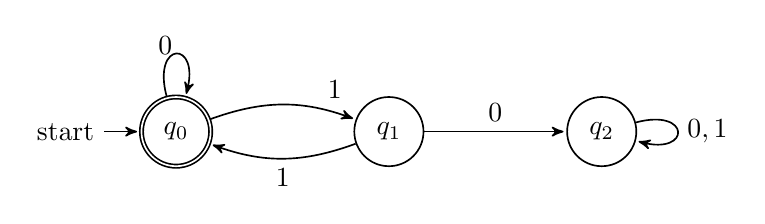
\begin{tikzpicture}[->,>=stealth',shorten >=1pt, auto, node distance=2cm, semithick]
\tikzstyle{every state}=[text=black, fill=none]

\node[initial,state, accepting] (q0)          {$q_0$};
\node[state]         (q1) [right of=q0, xshift=20pt] {$q_1$};
\node[state]         (q2) [right of=q1, xshift=20pt] {$q_2$};

\path (q0) edge  [loop above, near start] node {$0$} (q0)
        edge [bend left=20, near end] node {$1$} (q1)
    (q1) edge [bend left=0] node {$0$} (q2)
        edge [bend left=20] node {$1$} (q0)
    (q2) edge [loop right] node {$0,1$} (q2)
;
\end{tikzpicture}
\end{center}
where $Q = \{q_0, q_1, q_2\}$, $\Sigma = \{0,1\}$, and $F = \{q_0\}$, and $\delta: Q \times \Sigma \to Q$
is specified by the look-up table
\begin{center}
\begin{tabular}{c|cc}
        & $0$ & $1$ \\
    \hline
  $q_0$ & $q_0$ & $q_1$ \\
  $q_1$ & $q_2$ & $q_0$ \\
  $q_2$ & $q_2$ & $q_2$
\end{tabular}
\end{center}
    \begin{enumerate}
    \item\gradeComplete A friend tries to summarize the transition function with the formula
    \[
        \delta(q_i,x) = \begin{cases}
            q_0 &\text{ when $i=0$ and $x=0$} \\
            q_2 &\text{ when $x < i$}\\
            q_j &\text{ when $j = (i+1) \mod 2$ and $x=1$}
        \end{cases}
    \]
    for $x \in \{0,1\}$ and $i \in \{0,1,2\}$.
    Are they right? Either help them justify their claim or give a counterexample to disprove it and then 
    fix their formula.

    \item\gradeCorrect Give a regular expression $R$ so that $L(R)$ is the language 
    recognized by this finite automaton. Justify your answer by referring to the 
    definition of the semantics of regular expressions and computations of finite automata. 
    Include an explanation for why each string in $L(R)$ is accepted by the finite automaton {\it and}
    for why each string not in $L(R)$ is rejected by the finite automaton.

    \item\gradeCorrect Keeping the same set of states $Q = \{q_0, q_1, q_2\}$, alphabet $\Sigma = \{0,1\}$, 
    same start state $q_0$, and same transition 
    function $\delta$, choose a new set of accepting states $F_{new}$ so that the new 
    finite automaton that results accepts at least one string that the original one rejected {\bf and} rejects
    at least one string that the original one accepted, or explain why there is no such choice of $F_{new}$.
    A complete solution will include either (1) a precise and
    clear description of your choice of $F_{new}$
    and a precise and clear the two example strings using relevant definitions 
    to justify them, or (2) a sufficiently general and correct argument
    why there is no such example, referring back to the relevant definitions.

    \end{enumerate}
\item \textbf{Automata design} (12 points):
As background to this question, recall that integers can be represented using base $b$ expansions, for 
any convenient choice of base $b$. The precise definition is:
for $b$ an integer greater than $1$ and $n$ a positive integer, 
the {\bf base $b$ expansion of $n$}  is defined to be
\[
(a_{k-1} \cdots a_1 a_0)_b
\]
where $k$ is a positive integer, $a_0, a_1, \ldots, a_{k-1}$ 
are nonnegative integers less than $b$, $a_{k-1} \neq  0$, and
\[
n =  \sum_{i=0}^{k-1} a_{i} b^{i}
\]

Notice: {\it The base $b$ expansion of a positive integer $n$ is a string over the alphabet 
$\{x \in \mathbb{Z} \st 0 \leq x < b\}$
whose leftmost character is nonzero.}

An important property of base $b$ expansions of integers is that, for each integer $b$ greater than $1$,
each positive integer $n = (a_{k-1} \cdots a_1 a_0)_b$, and each nonnegative integer $a$ less than $b$, 
\[
    bn + a = (a_{k-1} \cdots a_1 a_0a)_b
\]
In other words, shifting the base $b$ expansion to the left results in multiplying the integer value by the base.
In this question we'll explore building deterministic finite automata that recognize 
languages that correspond to useful sets of integers.

    \begin{enumerate}
    \item\gradeCompleteFirst Design a DFA that recognizes the set of binary (base $2$) expansions of 
    positive integers that are powers of $2$. A complete solution will include the state diagram of your DFA and 
    a brief justification 
    of your construction by explaining the role each state plays in the machine, as well as a brief 
    justification about how the strings accepted and rejected by the machine connect to the specified language.

    {\it Hints}: (1) A power of $2$ is an integer $x$ that can be written as $2^y$ for some nonnegative integer $y$, 
    (2) the DFA should accept the strings $100$, $10$ and $100000$ and should reject the 
    strings $010$, $1101$, and $\varepsilon$ (can you see why?).

    \item\gradeComplete Consider arbitrary positive integer $m$. Design a DFA that recognizes the 
    set of binary (base $2$) expansions of positive integers that are multiples of $m$. A complete solution will
    include the formal definition of your DFA (paramterized by $m$) and a brief justification of your 
    construction by explaining the role each state plays in the machine, as well as a brief 
    justification about how the strings accepted and rejected by the machine connect to the specified language.

    {\it Hints}: (1) Consider having a state for each possible remainder upon division by $m$.
     (2) To determine transitions, notice that reading a new character will shift what we already read over by
     one slot.

    \item\gradeCorrectFirst Choose a positive integer $m_{0}$ between $5$ and $8$ (inclusive) and draw the state diagram
    of a DFA recognizing the following language over $\{0,1,2,3\}$ 
    $$\{ w \in \{0,1,2,3\}^* \mid w \text{ is a base $4$ expansion of a positive 
    integer that is a multiple of $m_0$}\}$$
    A complete solution will include the state diagram of your DFA and 
    a brief justification 
    of your construction by explaining the role each state plays in the machine, as well as a brief 
    justification about how the strings accepted and rejected by the machine connect to the specified language.
    \end{enumerate}

    {\it Bonus extension to think about (ungraded):} Which other languages related to sets of integers 
    can be proved to be regular using a similar strategy? 

\item \textbf{Nondeterminism} (15 points): For this question, the alphabet is $\{a,b\}$.
\begin{enumerate}
\item\gradeComplete Design a DFA that recognizes the language
    \[ 
    \{w \in \{a,b\}^* \mid w \text{ contains at most one $a$ {\bf and} at least two $b$s}\}
    \]
    You can design this DFA directly or use the constructions from class (and the footnote to Theorem 
    1.25 in the book) to build this DFA from DFA for the simpler languages that are intersected
    to give this language.
    
    A complete solution will include the state diagram of your DFA and 
    a brief justification 
    of your construction either by explaining the role each state plays in the machine, as well as a brief 
    justification about how the strings accepted and rejected by the machine connect to the specified language, 
    or by justifying the design of the DFA for the simpler languages and then describing how the Theorem was used.


    \item\gradeCorrect Design a NFA with at most $6$ states that recognizes the language
\[ 
\{w \in \{a,b\}^* \mid w \text{ contains at most one $a$ {\bf and} at least two $b$s}\}
\]
A complete solution will include the state diagram of your NFA and 
    a brief justification 
    of your construction by explaining the role each state plays in the machine, as well as a brief 
    justification about how the strings accepted and rejected by the machine connect to the specified language.
    Give one example string in the language and explain the computation of the NFA
    that witnesses that the machine accepts this string.
    Also, give one example string not in the language and explain why the NFA rejects this string.

\item\gradeCorrect Design a NFA with at most $6$ states that recognizes the language
\[ 
\{w \in \{a,b\}^* \mid w \text{ contains at most one $a$ {\bf or} at least two $b$s}\}
\]
A complete solution will include the state diagram of your NFA and 
    a brief justification 
    of your construction by explaining the role each state plays in the machine, as well as a brief 
    justification about how the strings accepted and rejected by the machine connect to the specified language.
    Give one example string in the language and explain the computation of the NFA
    that witnesses that the machine accepts this string.
    Also, give one example string not in the language and explain why the NFA rejects this string.
\end{enumerate}
{\it Bonus extension to think about (ungraded):} Did you need all $6$ states? Could you design DFA with $6$ states that recognize
each of these langauges?

\item\textbf{General constructions} (15 points):
In this question, you'll practice working with formal general constructions
for NFAs and translating between state diagrams and formal definitions.

\begin{enumerate}
\item\gradeCorrect Consider the following general construction: Let $N_1 = (Q, \Sigma, \delta_1, q_1, F_1)$ be a NFA
and assume that $q_0 \notin Q$.
Define the new NFA $N_2 = (Q \cup \{q_0\}, \Sigma, \delta_2, q_0, \{q_1\})$ where 
$$\delta_2: (Q \cup \{q_0\}) \times \Sigma_\varepsilon \to \mathcal{P} (Q \cup \{q_0\})$$ is defined by
\[
    \delta_2 (q,a) = \begin{cases}
        \{ q' \in Q \mid q \in \delta_1(q',a)\} &\text{if $q \in Q$, $a \in \Sigma_{\varepsilon}$} \\
        F_1 &\text{if $q =q_0$, $a = \varepsilon$}\\
        \emptyset &\text{if $q = q_0$, $a \in \Sigma$}
    \end{cases}
\]
Illustrate this construction by defining a specific example NFA $N_1$ and applying the 
construction above to create the new NFA $N_2$. Your example NFA should
\begin{itemize}
    \item Have exactly four states (all reachable from the start state),
    \item Accept at least one string and reject at least one string, and
    \item Not have any states labelled $q_0$.
\end{itemize}
Apply the construction above to create the new NFA. A complete submission 
will include the state diagram of your example NFA $N_1$ and the state diagram of the NFA $N_2$ resulting 
from this construction and a precise and clear description of $L(N_1)$ and $L(N_2)$, justified
by explaining the role each state plays in the machine, as well as a brief 
justification about how the strings accepted and rejected by the machine connect to the language.

\item 
In Week 2's review quiz, we saw the definition that a set $X$ is said to be 
{\bf closed under an operation} if, for any elements in
$X$, applying to them gives an element in $X$. For example, the set of
integers is closed under multiplication because if we take any two
integers, their product is also an integer .

Recall the definitions we have: 
For each language $L$ over the alphabet $\Sigma_1 = \{0,1\}$, we have the 
associated set of strings
  $$EXTEND(L) = \{ w \in \Sigma_1^* ~|~ w = uv \text{ for some strings } u \in L \text{ and } v \in \Sigma_1^* \}$$
We will prove that the collection of languages over $\{0,1\}$ that are each 
recognizable by some NFA is closed under the $EXTEND$ operation.

\begin{enumerate}
 
   \item \gradeComplete As a helpful tool in our construction\footnote{A result that is proved in 
   order to work towards a larger theorem is called a Lemma.}, prove that every NFA can be 
   converted to an equivalent one that has a single accept state. Note: this is exercise 1.11 in 
   the textbook.

   \item \gradeCorrect Prove that the collection of languages over $\{0,1\}$ that are each 
   recognizable by some NFA is closed under the $EXTEND$ operation. You can assume 
   that you are given a NFA with a single accept state $N = (Q, \{0,1\}, \delta, q_0, \{q_{acc}\})$
   and you need to define a new NFA, $N_{new} = (Q_{new}, \{0,1\}, \delta_{new}, q_{new}, F_{new})$,
    so that $L(N_{new}) = EXTEND(L(N))$. 

    A complete solution will include precise definitions for $Q_{new}, \delta_{new}, q_{new},$ and 
    $F_{new}$, as well as a 
    a brief justification 
    of your construction by explaining why these definitions work, referring 
    specifically to the definition of $EXTEND$ and to acceptance of NFA.

\end{enumerate}

\end{enumerate}
\item\textbf{Multiple representations} (8 points):
For any language $L \subseteq \Sigma^*$, recall that we define its \emph{complement} as 
$$\overline{L} := \Sigma^* - L = \{w \in \Sigma^* \mid w \notin L\}$$ That is, the complement of $L$ 
contains all and only those strings which are not in $L$. Our notation for regular expressions does not 
include the complement symbol. However, 
it turns out that the complement of a language described by a regular expression is guaranteed to also be describable by a 
(different) regular expression.\footnote{We'll see that this is connected to the 
result we proved in class that the complement of each language recognizable by a DFA is 
recognizable by a(nother) DFA.}

For example, over the alphabet $\Sigma = \{a,b\}$, the complement of the language described 
by the regular expression $\Sigma^* b$ is described by the regular expression $\varepsilon \cup \Sigma^*a$
because any string that does not end in $b$
must either be the empty string or end in $a$.

For each of the regular expressions $R$ over the alphabet $\Sigma = \{a,b\}$ below, write the regular 
expression for~$\overline{L(R)}$. Your regular expressions may use the symbols
$\varnothing$, $\varepsilon$, $a$, $b$, and the 
following operations to combine them: union, concatenation, 
and Kleene star.

Briefly justify why your solution for each part works by giving plain English descriptions of the language 
described by the regular expression and of its complement and connecting them to the regular 
expression via relevant definitions. An English description that is more 
detailed than simply negating the description in the original language will likely be helpful in the justification.

Alternatively, you can justify your solution by first designing a DFA that recognizes $L(R)$, 
using the construction from class and the book to modify this DFA to get a new DFA that recognizes~$\overline{L(R)}$, 
and then applying the constructions from class and the book to convert this new DFA to a regular expression.

For each part of the question, clearly state which approach you're taking and include enough intermediate
steps to illustrate your work.


\begin{enumerate}
    \item\gradeCorrect $(a \cup b)^*a(a \cup b)^*$
    \item\gradeCorrect $(a \cup b) (a \cup b) (a \cup b)$
\end{enumerate}


\item \textbf{Using general constructions} (16 points): Consider the NFA $N$ over $\{0,1,2\}$ with state diagram


   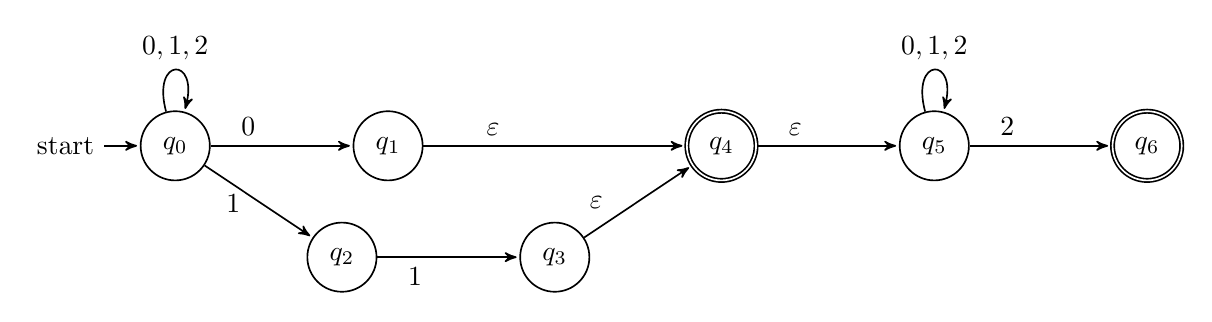
\begin{tikzpicture}[->,>=stealth',shorten >=1pt, auto, node distance=2cm, semithick]
   \tikzstyle{every state}=[text=black, fill=none]
   
   \node[initial,state] (q0)          {$q_0$};
   \node[state]         (q1) [right of=q0, xshift=20pt] {$q_1$};
   \node[state]         (q2) [below right of=q0, xshift=20pt] {$q_2$};
   \node[state]         (q3) [right of=q2, xshift=20pt] {$q_3$};
   \node[state, accepting]         (q4) [above right of=q3, xshift=20pt] {$q_4$};
   \node[state]         (q5) [right of=q4, xshift=20pt] {$q_5$};
   \node[state, accepting]         (q6) [right of=q5, xshift=20pt] {$q_6$};
   
   \path (q0) edge  [loop above] node {$0,1,2$} (q0)
           edge [bend right=0, near start] node[above] {$0$} (q1)
           edge [bend left=0, near start] node[below] {$1$} (q2)
       (q1) edge [bend left=0, near start] node {$\varepsilon$} (q4)
       (q2) edge [bend left=0, near start] node[below] {$1$} (q3)
       (q3) edge [bend left=0, near start] node {$\varepsilon$} (q4)
       (q4) edge [bend left=0, near start] node {$\varepsilon$} (q5)
       (q5) edge [loop above] node {$0,1,2$} (q5)
       (q5) edge [bend left=0, near start] node {$2$} (q6)
   ;
   \end{tikzpicture}

    \begin{enumerate}
      \item\gradeCompleteFirst Give two examples of strings of length greater than $2$ 
      that are accepted by $N$ and two examples of strings of length greater than $2$ 
      that are rejected by $N$. For each example string, list at least one of the 
      computations of $N$ on this string and 
      label whether this computation witnesses that the string is accepted by $N$.

      \item\gradeCorrectFirst Use the ``macro-state'' construction from Theorem 1.39 and class to create the DFA
      $M$ recognizing the same language as $N$. You only need to include states that are reachable from the start
      state. For full credit, submit (1) a state diagram that is deterministic (there should be arrows labelled $0$, $1$, and 
      $2$ coming out of each state) and where each state is labelled by a subset of the states in $N$; 
      and (2) for one of your example strings that is accepted by $N$, give the computation of $M$ on this string as a 
      seqeuence of states visited; and (3) for one of your example strings that is rejected by $N$, 
      give the computation of $M$ on this string as a seqeuence of states visited.

      \item\gradeComplete Give a mathematical description either using set builder notation or a regular expression
      for $L(N)$ and for $L(M)$.
    \end{enumerate}
\end{enumerate}
\newpage

\end{document}